\documentclass[border=5pt]{standalone}
\usepackage[T1]{fontenc}
\usepackage{tikz}

\definecolor{garnet}{HTML}{73000A}
\definecolor{atlantic}{HTML}{466A9F}
\definecolor{congaree}{HTML}{1F414D}
\definecolor{warmgrey}{HTML}{676156}
\definecolor{bk70}{HTML}{5C5C5C}
\definecolor{bk50}{HTML}{A2A2A2}
\definecolor{bk30}{HTML}{C7C7C7}
\definecolor{bk10}{HTML}{ECECEC}

\begin{document}
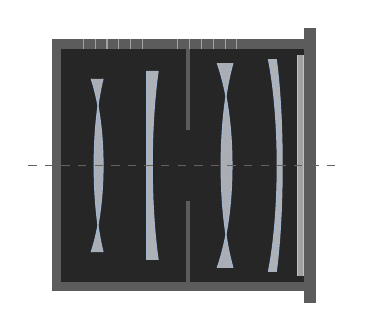
\begin{tikzpicture}

  % === Lens Assembly — cross-section side view ===
  % Light enters from the right, passes through elements, exits left toward sensor

  \def\barrelH{1.6}   % half-height of barrel
  \def\barrelL{3.2}    % barrel length

  % Barrel (outer housing)
  \fill[bk70] (0, -\barrelH) rectangle (\barrelL, -\barrelH + 0.12);
  \fill[bk70] (0, \barrelH - 0.12) rectangle (\barrelL, \barrelH);
  % Barrel end caps
  \fill[bk70] (0, -\barrelH) rectangle (0.12, \barrelH);

  % Barrel front (wider flare)
  \fill[bk70] (\barrelL, -\barrelH - 0.15) rectangle (\barrelL + 0.15, \barrelH + 0.15);

  % Focus ring texture (horizontal lines on barrel top)
  \foreach \x in {0.4,0.55,...,1.2} {
    \draw[bk50, line width=0.4pt] (\x, \barrelH - 0.12) -- (\x, \barrelH);
  }

  % Zoom ring texture
  \foreach \x in {1.6,1.75,...,2.4} {
    \draw[bk50, line width=0.4pt] (\x, \barrelH - 0.12) -- (\x, \barrelH);
  }

  % Interior cavity (dark)
  \fill[black!85] (0.12, -\barrelH + 0.12) rectangle (\barrelL, \barrelH - 0.12);

  % === Glass elements (convex/concave lens profiles) ===
  % Element 1: biconvex (near sensor side)
  \fill[atlantic!15, opacity=0.7]
    (0.5, -1.1) .. controls (0.7, -0.5) and (0.7, 0.5) .. (0.5, 1.1)
    -- (0.65, 1.1) .. controls (0.5, 0.5) and (0.5, -0.5) .. (0.65, -1.1) -- cycle;
  \draw[atlantic!50, thin]
    (0.5, -1.1) .. controls (0.7, -0.5) and (0.7, 0.5) .. (0.5, 1.1);
  \draw[atlantic!50, thin]
    (0.65, -1.1) .. controls (0.5, -0.5) and (0.5, 0.5) .. (0.65, 1.1);

  % Element 2: plano-concave
  \fill[atlantic!12, opacity=0.7]
    (1.2, -1.2) -- (1.2, 1.2)
    -- (1.35, 1.2) .. controls (1.25, 0.5) and (1.25, -0.5) .. (1.35, -1.2) -- cycle;
  \draw[atlantic!50, thin]
    (1.2, -1.2) -- (1.2, 1.2);
  \draw[atlantic!50, thin]
    (1.35, -1.2) .. controls (1.25, -0.5) and (1.25, 0.5) .. (1.35, 1.2);

  % Aperture stop (iris)
  \fill[bk70] (1.7, -1.48) rectangle (1.75, -0.45);
  \fill[bk70] (1.7, 0.45) rectangle (1.75, 1.48);

  % Element 3: biconvex (larger)
  \fill[atlantic!15, opacity=0.7]
    (2.1, -1.3) .. controls (2.35, -0.6) and (2.35, 0.6) .. (2.1, 1.3)
    -- (2.3, 1.3) .. controls (2.1, 0.6) and (2.1, -0.6) .. (2.3, -1.3) -- cycle;
  \draw[atlantic!50, thin]
    (2.1, -1.3) .. controls (2.35, -0.6) and (2.35, 0.6) .. (2.1, 1.3);
  \draw[atlantic!50, thin]
    (2.3, -1.3) .. controls (2.1, -0.6) and (2.1, 0.6) .. (2.3, 1.3);

  % Element 4: meniscus (near front)
  \fill[atlantic!12, opacity=0.7]
    (2.75, -1.35) .. controls (2.9, -0.6) and (2.9, 0.6) .. (2.75, 1.35)
    -- (2.85, 1.35) .. controls (2.95, 0.6) and (2.95, -0.6) .. (2.85, -1.35) -- cycle;
  \draw[atlantic!50, thin]
    (2.75, -1.35) .. controls (2.9, -0.6) and (2.9, 0.6) .. (2.75, 1.35);
  \draw[atlantic!50, thin]
    (2.85, -1.35) .. controls (2.95, -0.6) and (2.95, 0.6) .. (2.85, 1.35);

  % Front glass (flat protective element)
  \fill[atlantic!8, opacity=0.6]
    (\barrelL - 0.08, -1.4) rectangle (\barrelL, 1.4);
  \draw[atlantic!40, thin]
    (\barrelL - 0.08, -1.4) -- (\barrelL - 0.08, 1.4);
  \draw[atlantic!40, thin]
    (\barrelL, -1.4) -- (\barrelL, 1.4);

  % Optical axis (dashed)
  \draw[warmgrey, dashed, thin] (-0.3, 0) -- (\barrelL + 0.5, 0);

\end{tikzpicture}
\end{document}
